%% Common asset library for recurrent neural networks
%%
%% Modular images and common setup for tikz pictures
%%
\usepackage{graphicx}
\usepackage{xargs}
\usepackage{ifthen}
\usepackage{bm}

%% Tikz libraries
\usetikzlibrary{automata,arrows,shapes,matrix,trees,calc,fit,backgrounds,math}

%% Simple network nodes
\tikzset{
  ionode/.style n args={3}{
    circle, thick,
    minimum size=#1,
    inner sep=0pt,
    outer sep=0pt,
    draw=#2!80,
    fill=#2!20,
    label=center:#3,
  }
}
\tikzset{input/.style={ionode={16pt}{blue}{#1}}}
\tikzset{output/.style={ionode={16pt}{red}{#1}}}


%%%%%%%%%%%%%%%%%%%%%%%%%%%%%%%%%%%%%%%%%%%%%%%%%%
%% LSTM command
%%%%%%%%%%%%%%%%%%%%%%%%%%%%%%%%%%%%%%%%%%%%%%%%%%
%% Base on https://duckduckgo.com/?t=ffab&q=lstm+illustration&atb=v1-1&iax=images&ia=images&iai=https%3A%2F%2Fwww.herongyang.com%2FNeural-Network%2FLSTM-Long-Short-Term-Memory-github.png
\def\nodesep{0.8}
\def\consep{0.4}
\tikzset{
  pwiselabel/.style={
    white,
    font=\sffamily\bfseries\tiny
  }
}
\tikzset{
  pwise/.style={
    rectangle,
    inner sep=2.5pt,
    rounded corners=1pt,
    fill=black,
    label={[pwiselabel]center:#1}
  },
  vcon/.style={
    label={center:\tikz\draw[->, thick, >=latex'] (0, 0.2*#1) to[out=300, in=180] (0.2*#1, 0) to[out=180, in=60] (0, -0.2#1) to[out=60, in=180] (0.2*#1, 0) -- (0.5#1, 0);}
  },
  sigtan/.style n args={3}{
    circle,
    minimum size=#1,
    inner sep=0pt,
    fill=#2!80,
    label={center:\tikz\draw[white, thick]  (-#3, -#3) .. controls (#3, -#3) and (-#3, #3) .. (#3, #3);}
  },
  signode/.style={sigtan={12pt}{red}{3pt}},
  tanhnode/.style={sigtan={12pt}{blue}{3pt}},
  connode/.style={inner sep=0pt, outer sep=0pt, node distance=\consep cm},
}
\newcommand*{\lstm}{
  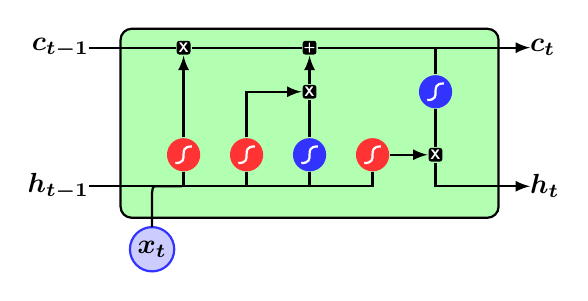
\begin{tikzpicture}[>=latex, thick, node distance=\nodesep cm]
    \draw[rounded corners, fill=green!30] (0,0) rectangle (6*\nodesep, 3*\nodesep);
    \node[signode] (s1) at (\nodesep, \nodesep) {};
    \node[signode, right of=s1] (s2) {};
    \node[pwise=X, above of=s1, node distance=1.7*\nodesep cm] (p1) {};
    \node[tanhnode, right of=s2] (t1) {};
    \node[signode, right of=t1] (s3) {};
    \node[pwise=X, right of=s3] (p2) {};
    \node[tanhnode, above of=p2] (t2) {};
    \node[pwise=X, above of=t1] (p3) {};
    \node[pwise=+, right of=p1, node distance=2*\nodesep cm] (p4) {};

    %% Cell state
    \node[connode, node distance=1.5*\nodesep cm, left of=p1, anchor=east] (ctminus1) {$\boldsymbol{c_{t-1}}$};
    \node[connode, node distance=3.5*\nodesep cm, right of=p4, anchor=west] (ct) {$\boldsymbol{c_t}$};
    \draw[shorten >= 0.2*\consep cm] (t2) |- (ct);
    \draw[->] (ctminus1) -- (p1) -- (p4) -- (ct);

    %% Input state
    \node[connode, below of=s1] (con1) {};
    \node[connode, left of=con1] (con2) {};

    \node[input={$\boldsymbol{x_t}$}, node distance=\nodesep cm, below of=con2] (xt) {};
    \draw (xt) -- ($ (xt) !.9! (con2) $) to [out=90, in=180] ($ (xt|-con1.east) !.1! (con1.east) $) -- (con1) -| (s1);

    %% Hidden state
    \node[connode, node distance=\consep * 2 cm, left of=con2, anchor=east] (htminus1) {$\boldsymbol{h_{t-1}}$};
    \node[connode, node distance=\nodesep * 6 cm, right of=con2, anchor=west] (ht) {$\boldsymbol{h_{t}}$};
    \draw (htminus1) -| (s1);
    \draw (htminus1) -| (t1);
    \draw (htminus1) -| (s2);
    \draw (htminus1) -| (s3);

    %% Remaining edges
    \draw[->] (s1) -- (p1);
    \draw[->] (s2) |- (p3);
    \draw (t1) -- (p3);
    \draw[->] (s3) -- (p2);
    \draw (p2) -- (t2);
    \draw[->] (p2) |- (ht);
    \draw[->] (p3) -- (p4);
    
  \end{tikzpicture}  
}

\newcommand*{\lstmforgetstate}{
   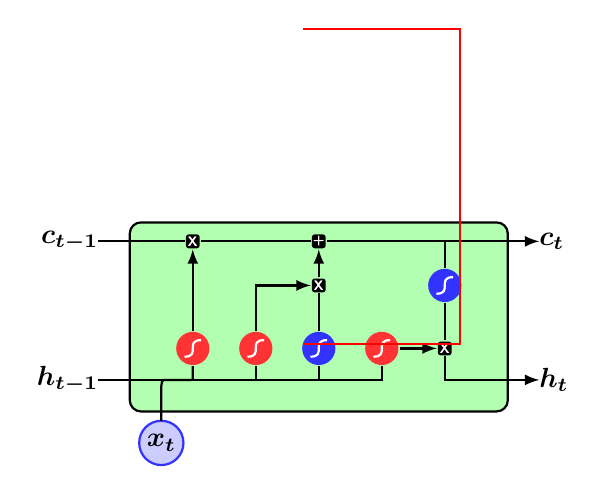
\begin{tikzpicture}[>=latex, thick, node distance=\nodesep cm]
     \node {\lstm};
     \draw[red] (0,0) -- (2,0) -- (2, 4) -- (0, 4);
   \end{tikzpicture}
 
}

%%%%%%%%%%%%%%%%%%%%%%%%%%%%%%%%%%%%%%%%%%%%%%%%%% 
%% GRU
%%%%%%%%%%%%%%%%%%%%%%%%%%%%%%%%%%%%%%%%%%%%%%%%%%
\newcommand*{\gru}{
  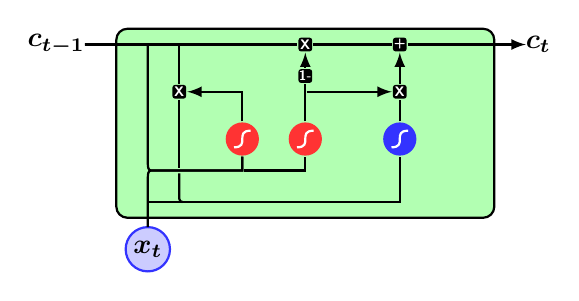
\begin{tikzpicture}[>=latex, thick, node distance=\nodesep cm]
    \draw[rounded corners, fill=green!30] (0,0) rectangle (6*\nodesep, 3*\nodesep);
    \node[signode] (s1) at (2*\nodesep, 1.25*\nodesep) {};
    \node[signode, right of=s1] (s2) {};
    \node[connode, above of=s1, node distance=1.5*\consep cm] (cs1p1) {};
    \node[pwise=X, left of=cs1p1] (p1) {};
    \node[pwise={1-}, above of=s2] (p2) {};
    \node[pwise={X}, above of=p2, node distance=\consep cm] (p3) {};
    \node[tanhnode, right of=s2, node distance=1.5*\nodesep cm] (t1) {};
    \node[pwise=X, above of=t1, node distance=1.5*\consep cm] (p4) {};
    \node[pwise=+, right of=p3, node distance=1.5*\nodesep cm] (p5) {};

    %% Invisible nodes
    \node[connode, above of=s2, node distance=1.5*\consep cm] (p2b) {};
    % Row 2
    \node[connode, below of=s1] (s32) {};
    \node[connode, left of=s32, node distance=\nodesep cm] (s22) {};
    \node[connode, left of=s22] (s12) {};

    % Row 1
    \node[connode, below of=s12] (s11) {};
    \node[connode, right of=s11] (s21) {};
    \node[connode, right of=s21] (s31) {};
    \node[connode, right of=s21, node distance=3*\nodesep cm] (s51) {};
    
    %% Input
    \node[input={$\boldsymbol{x_t}$}, node distance=.75*\nodesep cm, below of=s11] (xt) {};
    
    %% Cell state
    \node[connode, node distance=3.5*\nodesep cm, left of=p3, anchor=east] (ctminus1) {$\boldsymbol{c_{t-1}}$};
    \node[connode, node distance=2*\nodesep cm, right of=p5, anchor=west] (ct) {$\boldsymbol{c_t}$};
    \draw[->] (ctminus1) -- (p3) -- (p5) -- (ct);

    %% Edges
    
    % Tanh to +
    \draw[->] (p4) -- (p5);
    \draw (t1) -- (p4);

    % xt to t1 and others
    \draw (xt) |- (s11-|t1) -| (t1);
    \draw (xt) -- ($ (xt) !.9! (s12) $) to [out=90, in=180] ($ (xt|-s22.east) !.1! (s22.east) $) -| (s1);
    \draw (ctminus1) -| ($ (xt) !1.1! (s12) $) to [out=270, in=180] ($ (xt|-s22.east) !.1! (s22.east) $) -| (s1);
    \draw (s32) -| (s2);
    \draw[->] (s1) |- (p1);
    \draw (ctminus1) -| (p1);
    \draw[shorten >= 0.05*\consep cm] (p1) -- (s22);
    \draw[shorten <= 0.05*\consep cm] (s22) -- ($ (s22) !.9! (s21) $) to[out=270, in=180] ($ (s21) !.1! (s31) $);
    \draw (s2) -- (p2);
    \draw[->] (p2) -- (p3);
    \draw[->] (p2b) -- (p4);

  \end{tikzpicture}  
}
